\section{Experiments}
\def\experimentSnapshot{2026-11-05 04:08 UTC}

\paragraph{Execution snapshot.} At \experimentSnapshot, the original 856 configurations include 556 complete, 21 retained unfinished, 278 deferred, and 1 failed. The reduced scope is explicit in Appendix~\ref{app:reduced-scope}; deferred runs supply no evidence.
\paragraph{Protocol.} All runs use a single seed, seed 42. We therefore report long-run endpoints and curves as deterministic case studies, not as high-confidence statistical estimates. The revision recomputes configuration selection on validation criteria within each method (Appendix~\ref{app:revision-audit}); and the main comparison is against same-maximum-rank Single-Grassmann. PINN metrics are relative $L_2$ error where lower is better; classification and graph metrics are accuracies where higher is better.

\paragraph{Completed follow-up evidence.}
The completed PubMed/SAGE two-rate cohort gives STRATA test accuracy 0.71623, versus 0.67902 for Single-Grassmann and 0.69061 for AdamW: descriptive gains of 3.721 and 2.562 percentage points. Each method selects its rate using terminal-100 validation accuracy. Its archived optimizer tensor state, including fixed probes, is 58.1\% of AdamW's. Table~\ref{tab:pubmed-resources} gives all five methods, including stronger competitors; this is a comparison-specific benefit, not a graph-family or significance claim.
\begin{table*}[t]\centering\footnotesize
\caption{PubMed/SAGE: validation-selected two-rate, seed-42, 1000-epoch comparisons. State is unique optimizer tensor storage read from the final checkpoint, including probes. Peak is maximum recorded CUDA allocation; wall time is shared-server epoch timing, not isolated throughput.}\label{tab:pubmed-resources}
\begin{adjustbox}{max width=\linewidth}
\begin{tabular}{lrrrrr}\toprule Method & Val acc & Test acc & State MiB & Peak MiB & ms/epoch\\\midrule
\rowcolor{oursbg}
STRATA & 0.7179 & 0.7162 & 2.32 & 391.1 & 29.6 \\
Single-G & 0.7067 & 0.6790 & 1.82 & 390.6 & 24.2 \\
AdamW & 0.7041 & 0.6906 & 3.99 & 392.7 & \textbf{16.6} \\
GaLore & \textbf{0.7590} & \textbf{0.7580} & \textbf{1.26} & \textbf{390.0} & 22.3 \\
Independent & 0.7419 & 0.7415 & 2.20 & 391.0 & 27.3 \\
\bottomrule\end{tabular}
\end{adjustbox}\end{table*}
\begin{figure*}[t]\centering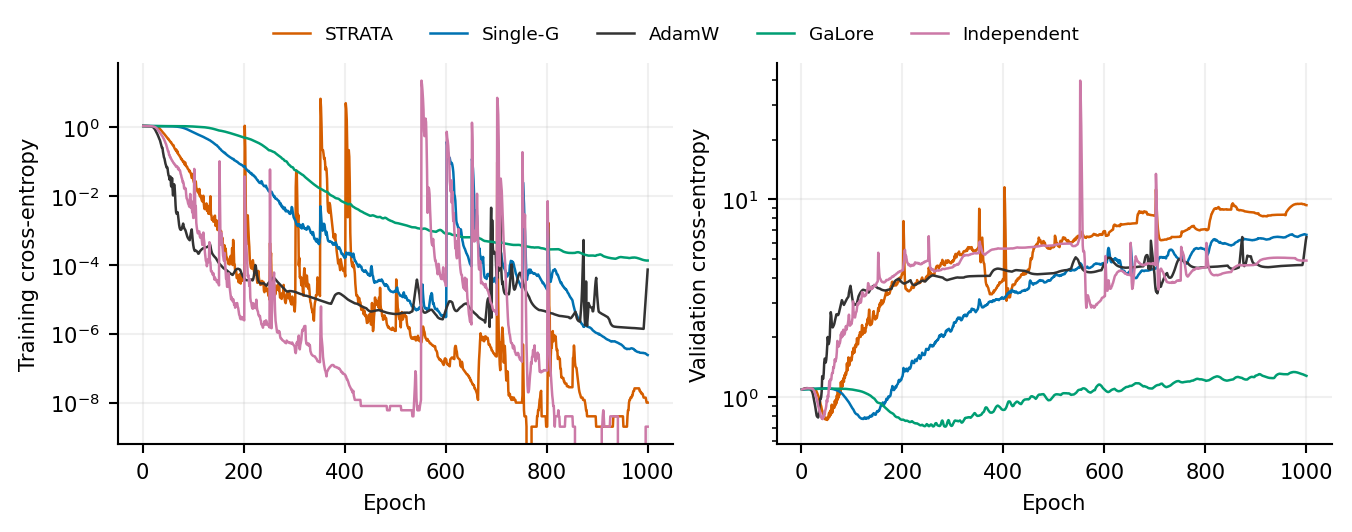
\includegraphics[width=.98\linewidth]{figures/fig_evidence_pubmed.png}\caption{Completed PubMed/SAGE training and validation trajectories. Each of five methods selects its learning rate using terminal-100 validation accuracy after both full-budget candidates finish. All trajectories are raw; held-out test outcomes are reported in Table~\ref{tab:pubmed-resources}.}\label{fig:pubmed-positive}\end{figure*}
The completed default-protocol PubMed architectures are gat, gcn, gcnii, sage; positive STRATA--Single-G test differences occur in gcn, sage. Every completed architecture remains in Table~\ref{tab:new-cohorts}. Further controlled ablations and an equal-budget flag-step sweep are reported in Appendix~\ref{app:evidence-extension}; experimental variants do not overwrite default-protocol results.
\paragraph{Mechanism evidence in the positive setting.} Both rates for all ten PubMed/SAGE interventions are complete (22 configurations including the full controls). Full STRATA reaches 71.623\%, exceeding every validation-selected ablation by 0.435--3.984 percentage points (Table~\ref{tab:pubmed-ablations}). This supports the combined configuration in this setting; interventions that also alter resets or the covariance objective do not isolate a single geometric cause.
\paragraph{Matched flag-step search.} In the completed exploratory six-candidate grid for each geometric method, validation selects STRATA at $\xi=10$ and $\eta=10^{-3}$, with test accuracy 73.383\%, versus 67.902\% for Single-Grassmann and 74.151\% for Independent. The STRATA--Single-G difference is 5.481 percentage points; STRATA improves by 1.760 points over its default-step result. Table~\ref{tab:xi-sweep} and the full profiles retain every setting. This is a separate sensitivity result, and Independent remains stronger on held-out test accuracy.
\paragraph{Equal-state follow-up.} A resource-only calibration selects Single-Grassmann rank 82, whose stored optimizer tensor state differs from STRATA R64 by -0.408\%. After the same six-candidate validation search for both methods, test accuracies are 73.383\% and 72.923\%, respectively (signed STRATA difference +0.460 percentage points; Table~\ref{tab:memory-control}). At the default flag step, the two-rate validation selections instead give STRATA 71.623\% and Single-G R82 72.923\%. Thus extra state is a material confound in the equal-rank comparison, and the retained six-grid gain is smaller and protocol-dependent.


\paragraph{Scope of the positive cases.}
Table~\ref{tab:positive-cases} collects three illustrative comparisons from the completed default graph matrix. These rows are chosen for exposition after observing the matrix; they are not a preselected confirmatory subset. Within every row, all methods finish both rates before validation selects a configuration. STRATA improves on Single-Grassmann in three of the twelve dataset--architecture settings, and does not in the other nine. The complete matrix and adverse cases appear in Appendix~\ref{app:full-empirical-record}. GaLore is stronger in these three cases, so they support restricted comparisons rather than a universal graph-optimizer ranking.
\begin{table*}[t]\centering\footnotesize\setlength{\tabcolsep}{3pt}
\caption{Illustrative positive same-rank comparisons, seed42, terminal-100 test accuracy after full two-rate validation selection. Every method is shown; higher is better. The full twelve-setting graph matrix is retained in the appendix.}
\label{tab:positive-cases}
\begin{adjustbox}{max width=\linewidth}
\begin{tabular}{lrrrrr}\toprule
Setting & STRATA & Single-G & AdamW & GaLore & Indep.\\\midrule
PubMed/SAGE & \cellcolor{oursbg}0.71623 & 0.67902 & 0.69061 & \textbf{0.75801} & 0.74151\\
PubMed/GCN & \cellcolor{oursbg}0.71742 & 0.71208 & 0.70445 & \textbf{0.75915} & 0.68782\\
CiteSeer/SAGE & \cellcolor{oursbg}0.55747 & 0.53980 & 0.55302 & \textbf{0.65124} & 0.55836\\
\bottomrule\end{tabular}
\end{adjustbox}\end{table*}
\paragraph{Other restricted benefits.}
The archived MNIST/MLP case gives STRATA accuracy 0.98273 versus Single-Grassmann 0.98011, while the available full-AdamW reference is about 0.987. Both completed five-method Rotated-MNIST grids below improve on Single-Grassmann after two-rate validation selection. In Poisson, STRATA has lower error than same-rank Single-Grassmann in an unstable baseline grid, while full AdamW is substantially better. These are specific vision, continual-learning and numerical-stability observations. They do not establish superiority over the strongest baseline across those families, and their complete adverse comparisons remain in the appendix.


\begin{table}[htbp]
\centering
\caption{\textbf{Numerical specification fixes.} The MNIST epsilon check is a diagnostic configuration; gradient norm and accuracy are the recorded values for that check.}
\label{tab:bugs}
\begin{adjustbox}{max width=\linewidth}
\begin{tabular}{lrrr}
\toprule
Projected $\epsilon$ & Max. $\|g\|$ & Test acc. $\uparrow$ & Separate counters \\
\midrule
$10^{-8}$ & $1.87\times10^5$ & 0.686 & -- \\
$10^{-6}$ & 14.2 & \textbf{0.969} & -- \\
\bottomrule
\end{tabular}
\end{adjustbox}
\end{table}
\begin{table}[htbp]
\centering
\caption{\textbf{Counter handling at a flag refresh.} Transported mature first moments and reinitialized second moments have different statistical ages.}
\label{tab:counter-fix}
\begin{adjustbox}{max width=\linewidth}
\begin{tabular}{lll}
\toprule
Rule & First-moment age & Second-moment age \\
\midrule
Shared reset & Reset despite transport & Reset \\
Separate counters & Retain mature age & Reset \\
\bottomrule
\end{tabular}
\end{adjustbox}
\end{table}


\paragraph{Numerical stability findings.} Tables~\ref{tab:bugs} and~\ref{tab:counter-fix} summarize the engineering contribution. The counter bug was diagnosed by observing gradient-norm oscillations synchronized with flag updates; transporting $M$ while resetting a shared counter made $\hat M$ roughly ten times too large after reset. The epsilon bug was diagnosed by decomposing update components: residual updates stayed bounded, while a flag-block Adam branch exploded because $V\approx0$ and epsilon was $10^{-8}$. On MNIST at the diagnostic setting, $\epsilon=10^{-8}$ produced max gradient norm $1.87\times10^5$ and test accuracy 0.686, while $\epsilon=10^{-6}$ produced max gradient norm 14.2 and test accuracy 0.969.

\paragraph{Memory/state accounting.} The revised tensor count includes both fixed probes and EMA sketches. For ranks $(16,32,64)$ and $p=8$, the STRATA/full-AdamW ratios for individual eligible matrices are 1.8125 for $128\times128$, 0.9063 for $256\times256$, 0.3393 for $784\times512$, 0.2070 for $512\times2048$, and 0.1035 for $4096\times1024$. Earlier reported model ratios excluded probes and are not treated as complete measured state. Archived peak-allocation logs show about 0.709 versus 0.772 GB on CIFAR, while STRATA takes about 24.2 versus 15.5 seconds per epoch; these small-model observations do not establish a large-model memory advantage. New runs retain actual tensor-state and peak-allocation measurements.

\paragraph{Completed continual-learning comparisons.} The Rotated-MNIST fine-tuning and replay grids each complete all ten candidates (five methods, two rates), with 1000 epochs across ten rotations, a two-layer 256-wide MLP, rank 64 and seed 42. Each method selects its rate by terminal-100 seen-task validation accuracy. In fine-tuning, STRATA attains 57.655\% test accuracy versus Single-Grassmann 57.109\% (+0.546 percentage points) and Independent 57.278\%; AdamW (62.193\%) and GaLore (59.691\%) remain stronger. With replay, STRATA reaches 88.582\%, above Single-Grassmann 87.170\% (+1.412 points) and Independent 87.140\%, while AdamW (90.720\%) and GaLore (88.880\%) remain higher. Thus both completed settings support a gain over Single-Grassmann, not an overall baseline ranking. Table~\ref{tab:new-cohorts} retains the full comparisons and replay protocol; Appendix~\ref{app:breadth-loss-updates} gives every selected loss trajectory. EWC remains deferred.

\paragraph{Tabular classification.} Completed 512-wide MLP grids give comparison-specific gains after all ten trials finish and each method selects its rate on validation. Red Wine Quality yields STRATA 71.500\% versus Single-Grassmann 69.702\% (+1.798 percentage points), with AdamW at 71.491\%. Adult gives 81.509\% versus Single-Grassmann 81.281\% (+0.227 points); AdamW and GaLore remain higher at 81.909\% and 81.838\%. Covertype gives 96.644\%, above AdamW's 96.448\% (+0.196 points) and GaLore's 96.597\%. Single-Grassmann is effectively tied at 96.642\%, while Independent is higher at 96.755\%. These are single-seed descriptive differences. The corresponding 256-wide models do not improve on Single-Grassmann. Table~\ref{tab:new-cohorts} retains all methods and completed settings; Appendix~\ref{app:breadth-loss-updates} gives the selected training and validation losses.

\paragraph{Token-budget language modeling.} The completed WikiText-103/GPT-2-small rank-16 grid gives STRATA test perplexity 144.54 versus GaLore 192.20, a 24.8\% reduction after two-rate validation selection. AdamW (80.00), Single-Grassmann (139.67), and Independent (140.81) remain stronger. Every candidate trains from scratch for 10000 updates and 20.48 million tokens, comprising 1000 ten-step evaluation units rather than corpus epochs. Table~\ref{tab:gpt2-complete} reports the full comparison and measured resources; Appendix~\ref{app:breadth-loss-updates} retains all selected loss trajectories.

\begin{table*}[t]\centering\footnotesize\setlength{\tabcolsep}{4pt}
\caption{\textbf{Completed new-task positive cases.} Terminal-100 test metrics after equal-count validation search. All five methods are shown; bold marks the best value. MSE/RMSE are lower-is-better and accuracy is higher-is-better. The full six-setting matrix and selected losses are in Appendix~\ref{app:new-family-results}.}
\label{tab:new-task-positive}\begin{adjustbox}{max width=\linewidth}
\begin{tabular}{llrrrrr}\toprule Setting & Metric & STRATA & Single-G & AdamW & GaLore & Indep.\\\midrule
ETTh2 / H24 & MSE & \cellcolor{oursbg}\textbf{1.74404} & 2.37970 & 2.16884 & 1.79170 & 2.18874 \\
MovieLens100K / ratings & RMSE & \cellcolor{oursbg}0.96949 & 1.00529 & \textbf{0.93295} & 0.95778 & 1.01755 \\
MovieLens1M / ratings & RMSE & \cellcolor{oursbg}1.05052 & 1.09444 & 0.98066 & \textbf{0.91712} & 1.08146 \\
Gas sensors / fine-tuning & acc & \cellcolor{oursbg}0.85453 & 0.85375 & 0.82335 & \textbf{0.90656} & 0.80659 \\
Gas sensors / replay & acc & \cellcolor{oursbg}0.96506 & 0.96409 & \textbf{0.96536} & 0.96232 & 0.96343 \\
\bottomrule\end{tabular}\end{adjustbox}\end{table*}
\paragraph{Transfer to forecasting, recommendation, and sensor drift.} All 180 configurations across six settings have completed their 1000-epoch budgets. Each of five methods selects among six candidates using terminal-100 validation metrics (Appendix~\ref{app:prospective-real-tasks}). STRATA improves on same-rank Single-Grassmann in 5/6 completed settings. Table~\ref{tab:new-task-positive} highlights these positive cases after observing the complete matrix; all settings, including ETTh1, appear in Table~\ref{tab:new-families-complete}. The results use seed 42 and describe the tested configurations.
\paragraph{Forecasting.} On ETTh2/H24, STRATA attains MSE 1.74404, the lowest among the five methods, reducing error by 26.7\%, 19.6\%, and 2.7\% relative to Single-Grassmann, AdamW, and GaLore, respectively. It stores 36.9\% of AdamW's optimizer tensor state. The common forecaster is an MLP; this comparison tests the optimizer under the specified chronological split.
\paragraph{Recommendation.} STRATA reduces RMSE relative to Single-Grassmann by 3.56\% on MovieLens100K and 4.01\% on MovieLens1M. AdamW and GaLore remain stronger on both datasets.
\paragraph{Sensor drift.} Fine-tuning gives 85.453\% accuracy, 3.118 percentage points above AdamW, while GaLore is stronger. With replay, STRATA reaches 96.506\%, versus AdamW's 96.536\%, using 55.1\% of its stored optimizer state. State counts include probes and buffers. These same-rank comparisons do not equalize geometric-method state, and stored-state savings do not imply peak-memory or throughput gains.

